\documentclass[11pt]{article}
%\documentclass[aps,preprint,superscriptaddress,11pt]{revtex4-1}
%\renewcommand{\familydefault}{\sfdefault}
%\usepackage{arial}
%\usepackage{arial}
%\renewcommand{\familydefault}{\sfdefault}

\renewcommand{\rmdefault}{phv} % Arial
\renewcommand{\sfdefault}{phv} % Arial
\usepackage[pdftex]{graphicx}
\usepackage{scrextend}
\usepackage{hyperref}

\usepackage{enumitem}
\setlist[1]{itemsep=-3pt,topsep=-3pt}

% Include figure files
\usepackage{bm}
\usepackage{graphicx}
\usepackage{subfig}
\usepackage{lscape}
\usepackage{empheq}
\usepackage[usenames,dvipsnames]{color}
%\usepackage[framemethod=tikz]{mdframed}                                                                                                     
\usepackage{amsfonts}
\usepackage{amsmath}
\usepackage{amsthm}
\usepackage{multirow}
\usepackage{bbold}
\usepackage[varg]{txfonts}
\usepackage{feynmp}
\DeclareGraphicsRule{*}{mps}{*}{}
\definecolor{eqcolor}{gray}{.9}
\usepackage{todonotes}

%\usepackage[justification=justified]{caption}
\usepackage{dcolumn}% Align table columns on decimal point
\usepackage{bm}% bold math
\usepackage{color}
\usepackage{subfig}
\usepackage{xspace}
\usepackage{lineno}
\usepackage{hyperref}% add hypertext capabilities
\usepackage{natbib}
\usepackage{ulem}
\usepackage{multicol}
\usepackage{eurosym}
\usepackage{enumitem}
\usepackage{setspace}
%\usepackage[mathlines]{lineno}% Enable numbering of text and display math
\usepackage[utf8]{inputenc}

%\RequirePackage{lineno}
%\linenumbers\relax % Commence numbering lines
\input symbols
\setlength
\linenumbersep{0.1cm}
%\linenumbers\relax % Commence numbering lines
%\usepackage[showframe,%Uncomment any one of the following lines to test 
%%scale=0.7, marginratio={1:1, 2:3}, ignoreall,% default settings
%%text={7in,10in},centering,
%%margin=1.5in,
%%total={6.5in,8.75in}, top=1.2in, left=0.9in, includefoot,
%%height=10in,a5paper,hmargin={3cm,0.8in},
%]{geometry}

%% page setup
\setlength{\hoffset}{-14mm}  
\setlength{\voffset}{-10mm}
\setlength{\textwidth}{175mm}
\setlength{\oddsidemargin}{12mm}
%\setlength{\textheight}{247mm}
\setlength{\textheight}{237mm}
\setlength{\topmargin}{-25mm}
\setlength{\headheight}{20mm}
\setlength{\headsep}{5mm}
\setlength{\footskip}{13mm}
\newlength{\capindent}
\setlength{\capindent}{1.0cm}
\newlength{\capwidth}
\setlength{\capwidth}{\textwidth}
\addtolength{\capwidth}{-2\capindent}

%% colours (see http://en.wikibooks.org/wiki/LaTeX/Colors) and fonts
\newcommand\introTitleColor{\color{Cerulean}}
\definecolor{darkmidnightblue}{rgb}{0.0, 0.2, 0.4}
%\newcommand\hkTitleColor{\color{BlueViolet}}
\newcommand\hkTitleColor{\color{darkmidnightblue}}
\definecolor{americanrose}{rgb}{1.0, 0.01, 0.24}
\newcommand\hkCommentColor{\color{americanrose}}
\definecolor{mediumred-violet}{rgb}{0.73, 0.2, 0.52}
\renewcommand*{\familydefault}{\sfdefault}
\newcommand\introNewParagraph{
  \smallskip
  \noindent
}
%%%
\newcommand{\FHC}{\ensuremath{\nu}-mode\xspace}
\newcommand{\RHC}{\ensuremath{\overline{\nu}}-mode\xspace}

\renewcommand{\baselinestretch}{1.}\normalsize

\begin{document}

\pagenumbering{roman}
\setcounter{page}{1}

%\newcommand{\thetacerenkov}{$\theta_{\mathrm{Cerenkov}}$}

%\graphicspath{{img/}}
%
\begin{flushright}
%\today\\
September 5, 2016\\
\end{flushright}
\vspace{5ex}
\centerline{\introTitleColor\Huge \bf Statement of Interest}
\centerline{\introTitleColor\Huge \bf for the Hyper-Kamiokande Experiment}
%
\vspace{5ex}
\bigskip

%\begin{center}
%{\introTitleColor\Large\bf HyperK}\\
P.\ Beltrame, 
G.A.\ Cowan, 
M.\ Needham, 
S.\ Playfer, 
G.\ Sidiropoulos 
(University of Edinburgh); 
P.\ Dunne,
P.\ Jonsson,
P.\ Litchfield,
Y.\ Uchida, 
M.O.\ Wascko 
(Imperial College London); 
T.\ Dealtry, 
A.\ Finch, 
L.\ Kormos, 
H.\ O'Keeffe (Lancaster University);
C.\ Andreopoulos, 
N.\ McCauley, 
D.\ Payne, 
J.\ Rose (University of Liverpool); 
G.\ Barr, 
D.\ Wark 
(University of Oxford); 
F.\ Di Lodovico, 
K.\ Hayrapetyan,
T.\ Katori,
A.\ Owen, 
R.\ Sacco, 
S.\ Short, 
R.\ Terri, 
J.\ Wilson,
B.\ Richards 
 (Queen Mary University of London); 
T.\ Berry, 
A.\ Kaboth,
J.\ Monroe 
(Royal Holloway University of London);
S.\ Cartwright, 
M.\ Malek, 
J.\ Perkin, 
L.\ Thompson (University of Sheffield); 
C.\ Densham, 
M.\ Fitton, 
T.\ Davenne, 
T.\ Nicholls, 
T.\ Stewart, 
M.\ Thorpe, 
A.\ Weber  
(STFC/RAL); 
G.\ Barker, 
S.\ Boyd, 
D. Hadley (University of Warwick).
%\end{center}

\vspace{5ex}
%
%
%
%\thispagestyle{empty}
\hspace{0.5cm}
\begin{figure}[htb]
\begin{center}
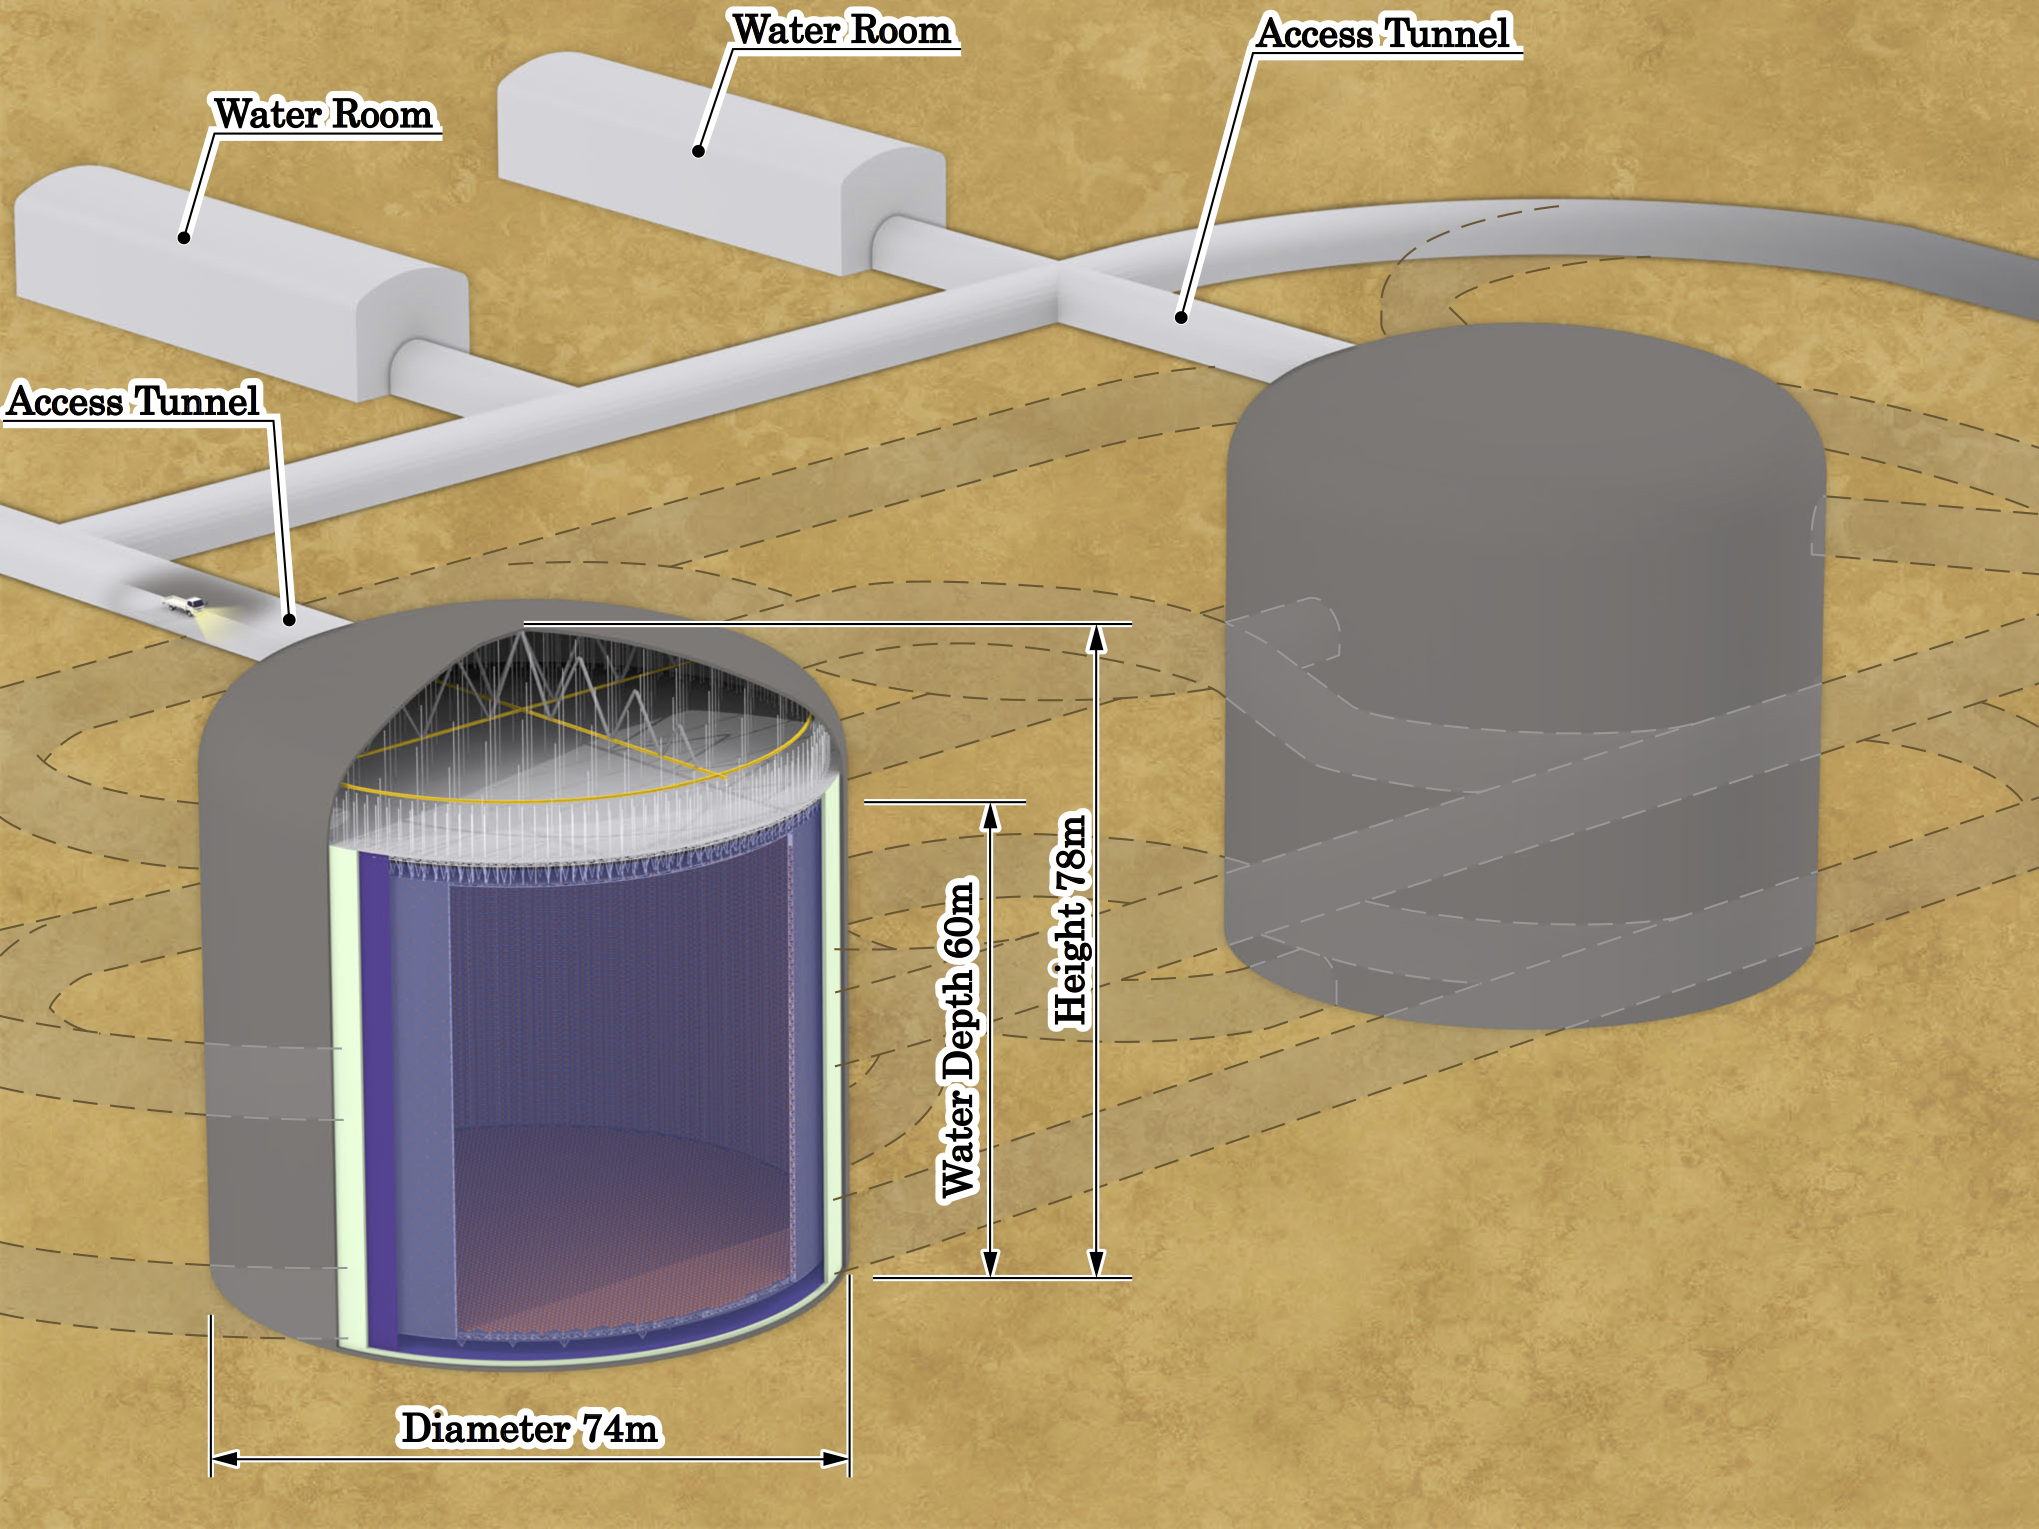
\includegraphics[scale=0.25]{figs/hyperk.png}
%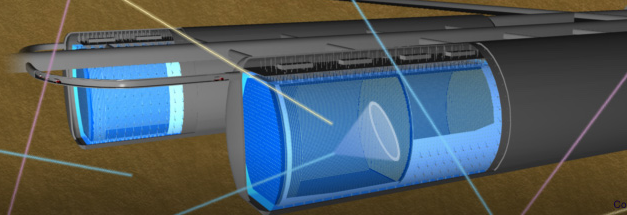
\includegraphics[scale=.7]{figs/hyperk-main.png}
\end{center}
%%\vspace{-3.5cm}
\end{figure}

\hspace{0.1cm}
\vspace{1ex}

\begin{figure}[htb]
\begin{center}

\includegraphics[scale=.4]{figs/edinburgh.jpg}
\vspace{.2cm}

\includegraphics[scale=0.4]{figs/ic.jpg}
\vspace{.2cm}

\includegraphics[scale=.4]{figs/lancaster.png}
\vspace{.2cm}

\includegraphics[scale=.3]{figs/liverpool.jpg}
\vspace{.2cm}

\includegraphics[scale=0.15]{figs/oxford.png}
\vspace{.2cm}\\

\includegraphics[scale=.4]{figs/qmul.jpg}
\vspace{.2cm}

\includegraphics[scale=.2]{figs/rhul.jpg}
\vspace{.2cm}

\includegraphics[scale=0.3]{figs/sheffield.png}
\hspace{.2cm}

\includegraphics[scale=0.5]{figs/RAL.png}
\vspace{.2cm}

\includegraphics[scale=.2]{figs/warwick.jpg}
\end{center}
%%\vspace{-3.5cm}
\end{figure}
\newpage

\makeatletter
\let\toc@pre\relax
\let\toc@post\relax
\makeatother

\newpage

%\tableofcontents
%%%%%%%%%%%%%%%%%%%%%%%%%%%%%%%%%%%%%%%%%%%%%%%%%%%%%%%%%%%%%%%%%%%%%%%%%%
\newpage
\pagenumbering{arabic}
\setcounter{page}{1}
\label{sec:hyperk}
\it{2 pages long text}

 
%\newpage
\bibliographystyle{unsrt}
\bibliographystyle{apsrev4-1}
\bibliography{mainfile}% Produces the bibliography via BibTeX.  

\end{document}
